\scanpage{6}
\[
\begin{aligned}
(P/Q)'&=\frac{P'}{Q}-P\frac{Q'}{Q^2}=\frac{P'Q-Q'P}{Q^2}\\
(P/Q)''&=P''/Q\deleted{\unsure{+}}\unsure{-|+}2\frac{P'Q'}{Q^2}+\deleted{\unsure{2}}P\bigl(
\end{aligned}
\]
\[
\frac{P'}{\deleted{Q}P}-\frac{Q'}{Q}
\qquad (xy)^{\unsure{2|''}}=\unsure{x''|x^2}y+2x'y^{\unsure{\prime}}+xy^{\unsure{\prime\prime|\prime}}
\]
% Detached point at full-scan (969,601), below/between the logarithmic quotients.
% Its layer, hand, and function are undetermined; the point is preserved without an inferred connection.
\margin{$\unsure{\cdot}$}
\[
\left(\frac{\deleted{\unsure{P'}}f}{g}\right)'=\frac{f'g-g'f}{g^2}
\]
\[
\frac{(P''Q+\deleted{P'Q'}-\deleted{P'Q'}\deleted{\unsure{+}}\unsure{-|+}Q''P)\unsure{Q^{\,2}|\deleted{Q}^{\,2}}
 -(P'Q-Q'P)2\deleted{Q}Q'}{Q^3}
\]
% The extra short rule below the right part of the next numerator reproduces
% a separate near-parallel ink stroke. Its intention is undetermined.
\[
\frac{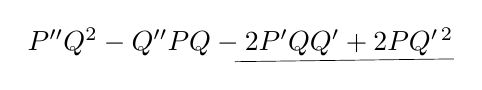
\begin{tikzpicture}[baseline=(num.base)]
\node[inner sep=0pt] (num) {$P''Q^2-Q''PQ-\unsure{2}P'QQ'+2PQ'^{\,2}$};
\draw[line width=.25pt] ([xshift=-2pt,yshift=-2pt]num.south) -- ([yshift=-1pt]num.south east);
\end{tikzpicture}}{Q^3}
\]
\[
2p^2Q^2\bigl(-\frac{Q'}{Q}+
\]

% The following layer is written after a half-turn and crossed by two long diagonal strokes.
\[
\deleted{\det\begin{pmatrix}a\deleted{\unsure{d|b}}&c\\b&d\end{pmatrix}-ad-bc\quad\text{inversible}}
\]
\[
\deleted{\begin{aligned}
&\delta(e_1e_{d-2})=-e_1\delta(e_{d-2})=-e_1e_{d-3}\deleted{=e_d}\\
&\qquad\rotatebox{90}{$=$}\\
&\delta(a\eta)=a\delta\eta=a\alpha e_{d-2}+a\beta f_{d-2}
\end{aligned}}
\]
\[
\deleted{\begin{aligned}
&\delta(e_1f_{d-2})=-\deleted{\unsure{f}}e_1\cdot f_{d-3}\\
&\qquad\rotatebox{90}{$=$}\\
&b\alpha e_{d-2}+b\beta f_{d-2}
\end{aligned}}
\]
\[
\deleted{\begin{aligned}
&\delta(f_1e_{d-2})=\delta(f_1)e_{d-2}-f_1\delta(e_{d-2})=e_{d-2}-f_1e_{d-3}\\
&\qquad\rotatebox{90}{$=$}\\
&\delta(c\eta)=c\delta\eta=c\alpha e_{d-2}+c\beta f_{d-2}
\end{aligned}}
\]
\deleted{etc}

\deleted{On en tire $e_1e_{d-3}$, $\deleted{\unsure{f}}e_1f_{d-3}$, $f_1e_{d-3}$, $f_1f_{d-3}$ comme comb. lin des $e_{d-1}$ et $f_{d-2}$, à coeff entiers fonctions de $\alpha,\beta$, $a,b,c,d$}

\[
\deleted{\begin{aligned}
&\delta(e_1x_i)=-e_1\delta(x_i)=-e_1\deleted{\unsure{\delta}}x_{i-1}\qquad 2\leq i\leq{}\\
&\qquad\rotatebox{90}{$=$}\\
&\delta(\deleted{\unsure{S}}s e_{i+1}+t f_{i+1})=s e_i+t f_i
\end{aligned}}
\]
% archive sheet number: 5
